
\chapter{System Evaluation}
\label{chapter:evaluation}

The system was used and tested on patients with cardiac diseases from Hospital de Santa Marta - CHLC (Lisbon) and the main variables collected were heart rate (HR) and Metabolic Equivalent of Tasks (METs) \cite{crouter_METS}. These variables were indicated by the hospital's cardiology team as being common variables used in their practice to diagnose and track patients \cite{importancia_HR_METS, importancia_HR_METS_2}. Variables to be collected determined the type of sensors needed.

Devices utilized to test this system were chosen as they provide cost effective platforms to support the desired functions. Cost and quality were taken into account and established market products were preferred as they offer greater consistency in quality over time and over numbers i.e. it is easy to ensure the good working of the system even if more devices are added after some time and they can be added in larger numbers to use with more patients.

\begin{figure}[!h]
	\centering
	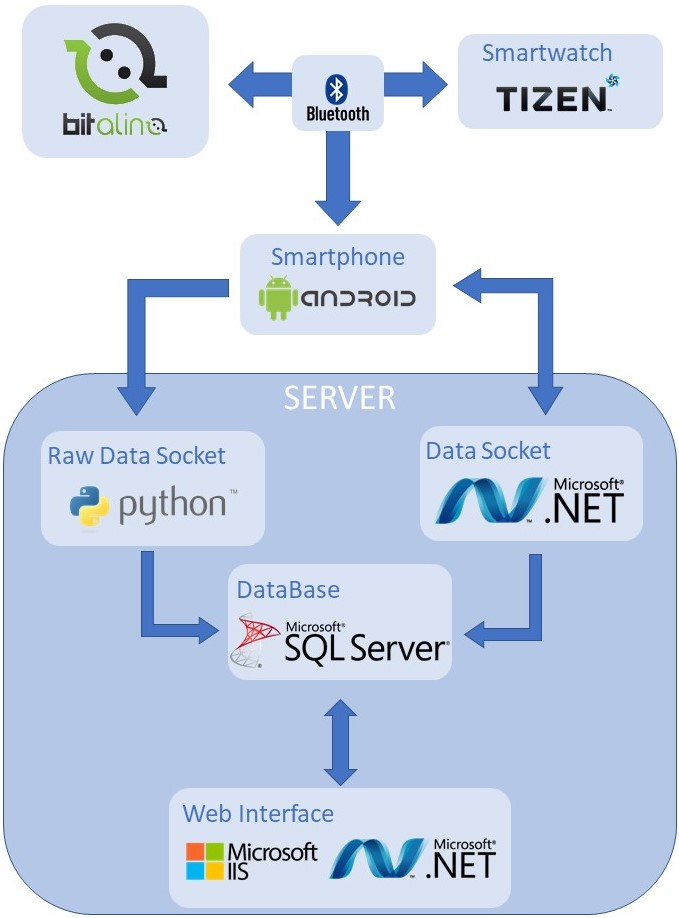
\includegraphics[width=0.75\textwidth]{platforms.jpg}
	\caption{Platforms and programing languages used to build and run the system. Choice of platforms were based on device}
	\label{fig:platforms}
\end{figure}

After all hardware and software was finished the system was tested in lab and hospital conditions. The main objectives of the tests were to assess system's usability, concerning comfort and ease of use by patient and doctor. Another major objective of testing the system was to verify the accuracy and reliability of the sensors utilized and the robustness of all the software, data transmissions and storage. All the software components were tested individually but still real life situations brought to light some minor bugs that were corrected once detected. Another major concern to be tested was loss of data during transmissions.

The devices used in the present work are directed to patients diagnosed or with suspects of cardiac insufficiency, hence the most relevant variables to collect are related with heart rate (HR) and accelerometry as a way of estimating the level of physical activity during the patients' daily life. To collect this data 3 devices were used, each with different sensors as detailed in \cref{table:vars}. Complete system architecture for the testing phase is depicted in \cref{fig:platforms}.

\begin{table}[!h]
	\centering
	\caption{Variables acquired by each device and the corresponding information extracted. 
		CD - Chest Deflection (respiratory frequency); PA - Physical Activity (measured in METs); ACC - Accelerometry}
	\label{table:vars}
	\begin{tabular}{|c|c|c|c|}
		\hline
		\textbf{Device } & \textbf{Variables} & \textbf{Sampling Rate (Hz)} & \textbf{Extracted information} \\ \hline
		\multirow{3}{*}{Smartwatch} & PPG       & 25                 & HR                    \\ \cline{2-4} 
		& HR        & 25                 & HR                    \\ \cline{2-4} 
		& ACC       & 100                & PA                    \\ \hline
		\multirow{3}{*}{BITalino}   & ECG       & 1000               & HR                    \\ \cline{2-4} 
		& ACC       & 1000               & PA                    \\ \cline{2-4} 
		& CD        & 1000               & RR                    \\ \hline
		Smartphone                  & ACC       & 100                & PA                    \\ \hline
	\end{tabular}
\end{table}

\FloatBarrier

\section{Wearable Sensors}

\subsection{Smartwatch}

The smartwatch used was the Samsung Gear S3 and it's function is to collect data and send it to the smartphone, acting like a sensor. This device was chosen as a way to reduce the patient's discomfort, as it can be a less invasive sensor, replacing the watch  many use daily. Another reason for the choice of this device was its novelty, as it was a new model at the time devices were chosen for this work, and it was expected to perform better than every previous smartwatch. Finally, the choice of this highly capable and versatile smart device was made with future developments in mind as it allowed for more functionalities to be implemented, like its use as a data hub (replacing the smartphone) and even allowing for an interface so the patient could interact with the system using only the smartwatch.
It has several sensors, including luminosity, atmospheric pressure, PPG, ACC and others decribed in \cite{Tizen_sensor}. %https://developer.tizen.org/development/api-references/native-application?redirect=/dev-guide/2.3.1/org.tizen.native.mobile.apireference/group__CAPI__SYSTEM__SENSOR__MODULE.html#ga41397923efb60755882608685edf1ecb
This device also has another "sensor" that produces values of instantaneous HR calculated from PPG data.

\subsubsection{Tizen App}

A native application software was developed to collect data from the desired sensors and send it, through BT, to the smartphone.
This smartwach's operative system (OS), Tizen, supports applications written in C language using many functions provided specifically for this OS.

When app is first initialized, a Bluetooth server is mounted awaiting for incoming connection from the smartphone. To prevent app being interrupted when screen is off, it is needed to lock CPU in on state and also, initialize sensors API with the appropriate option.

Code responsible for initializing the app Bluetooth server and sensors with the correct formulaion to prevent unintentional deactivation:

\bigskip
\begin{lstlisting}[language=C++]
#include <bluetooth.h>
#include <app_control.h>
#include <glib.h>
#include <stdlib.h>

static bool app_create(void *data){
	int server_socket_fd = -1;
	bt_adapter_state_e bt_ad_state = BT_ADAPTER_DISABLED;
	
	device_power_request_lock( POWER_LOCK_CPU, 0);
	
	bt_initialize();
	bt_adapter_get_state(&bt_ad_state);
	
	if (bt_ad_state != BT_ADAPTER_DISABLED) {
	} else {			
		bt_socket_create_rfcomm(BT_MGR_UUID, &server_socket_fd);
		bt_socket_set_connection_state_changed_cb(_socket_conn_state_changed_cb);
		bt_socket_listen_and_accept_rfcomm(server_socket_fd, MAX_NUM_PENDING);
	}
	
	data_initialize(data, update_sensor_values);

	if(feedback_initialize() == FEEDBACK_ERROR_NONE){
		feedback_play_type(FEEDBACK_TYPE_VIBRATION ,FEEDBACK_PATTERN_LOWBATT);
		feedback_play_type(FEEDBACK_TYPE_VIBRATION ,FEEDBACK_PATTERN_BT_CONNECTED);
		feedback_play_type(FEEDBACK_TYPE_VIBRATION ,FEEDBACK_PATTERN_BT_DISCONNECTED);
		feedback_play(FEEDBACK_PATTERN_LOWBATT);
		feedback_play(FEEDBACK_PATTERN_BT_CONNECTED);
		feedback_play(FEEDBACK_PATTERN_BT_DISCONNECTED);
	}

	return true;

}

bool data_initialize(void *data, Update_Sensor_Values_Cb sensor_update_cb)
{
	int i=0;
	
	//sensor_type_e sensors_list[] = {SENSOR_ACCELEROMETER, SENSOR_LIGHT, SENSOR_PRESSURE, SENSOR_HRM, SENSOR_HRM_LED_GREEN};

	sensor_type_e sensors_list[] = {SENSOR_ACCELEROMETER, SENSOR_HRM, SENSOR_HRM_LED_GREEN};

	for (i = 0; i < SENSOR_COUNT; ++i) {
		sensor_get_default_sensor(sensors_list[i], &sensors[i].handle);
		sensor_create_listener(sensors[i].handle, &sensors[i].listener);
		sensor_listener_set_option(sensors[i].listener, SENSOR_OPTION_ALWAYS_ON);
		sensor_listener_set_event_cb(sensors[i].listener, LISTENER_TIMEOUT, sensor_update_cb, i);
		sensor_listener_start(sensors[i].listener);
	}
	return true;
}

void update_sensor_values(int count, float *values, sensor_type_e type, appdata_s *ad)
{

// Manipulate sensor's values

}
\end{lstlisting}
\bigskip

When a Bluetoth connection is established, a particular message 'go' must be sent to initialize data collection. Other messages are available to stop the acquisition 'quit' or to request battery information 'batt'.

Code used to get battery status and percentage:

\bigskip
\begin{lstlisting}[language=C++]

device_battery_level_e battery_status = DEVICE_BATTERY_LEVEL_EMPTY;

int battery_percent = 0;

device_battery_get_percent(&battery_percent)

device_battery_get_level_status (&battery_status)

\end{lstlisting}
\bigskip

To interact with the sensors, a manufacturer provided API was used. It is built in a logic of callbacks, i.e. an event is generated when the sensor value changes.
Sampling rate is defined to be the default for each sensor that, according with the manufacturer guide, can range between 100Hz and 1 HZ \cite{Tizen_sensor} meaning that events occur at different rates for different sensors. 

To have a uniform sampling protocol, a buffer is kept containing the current value of each sensor and whenever a sensor event occurs, the corresponding values in this buffer are updated. In parallel, in another thread, there is a timer running at 100Hz that takes a snapshot of values in the buffer and writes them into a different array accompanied by a timestamp of the moment the snapshot was taken. Data from all sensors is held and when the array has 10 seconds of data, it is sent to the smartphone. This transmission strategy was implemented as a way of reducing the overhead of sending samples in real time, at 100Hz, which had a larger battery consumption and also induced the loss of samples, reported by the BT API provided by the manufacturer, returning an error for every message lost. The buffer technique was used as a very easy and simple way of upsampling data from sensors with a sampling frequency lower than 100Hz using a sample and hold method.

\begin{figure}[!h]
	\centering
	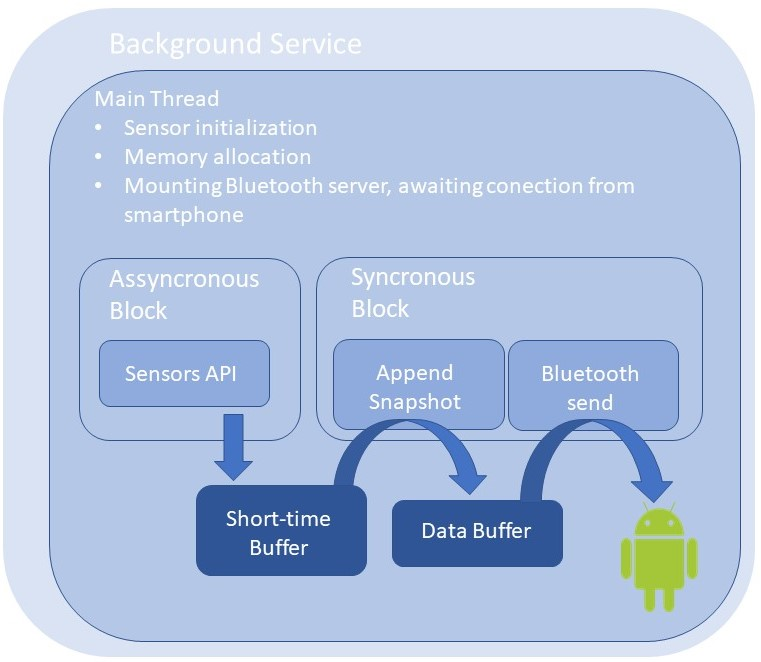
\includegraphics[width=0.75\textwidth]{app_tizen.jpg}
	\caption{Smartwatch App threads call-stack}
	\label{fig:app_tizen}
\end{figure}

\Cref{fig:app_tizen} shows the implemented app architecture having two main components, an asynchronous and synchronous block. The first runs when a sensor reports a new sample and its callback ir triggered. This function updates the buffer value that corresponds to the sensrs that triggered its callback. The other block that runs periodically and appends the current buffer values to another, larger, array, that stores 10s of data. This block is also responsible for sending the data when the 10s of data is collected, clearing the storage array.

%https://developer.tizen.org/development/api-references/native-application?redirect=/dev-guide/2.3.1/org.tizen.native.mobile.apireference/group__CAPI__SYSTEM__SENSOR__MODULE.html

%https://developer.tizen.org/development/api-references/native-application?redirect=https://developer.tizen.org/dev-guide/2.3.1/org.tizen.native.mobile.apireference/group__CAPI__SYSTEM__SENSOR__INFORMATION__MODULE.html

%http://www.mdpi.com/2075-4426/7/2/3/html

%https://news.samsung.com/global/in-depth-look-the-parts-and-pieces-that-make-the-gear-s3-tick

\begin{figure}[!h]
	\centering
	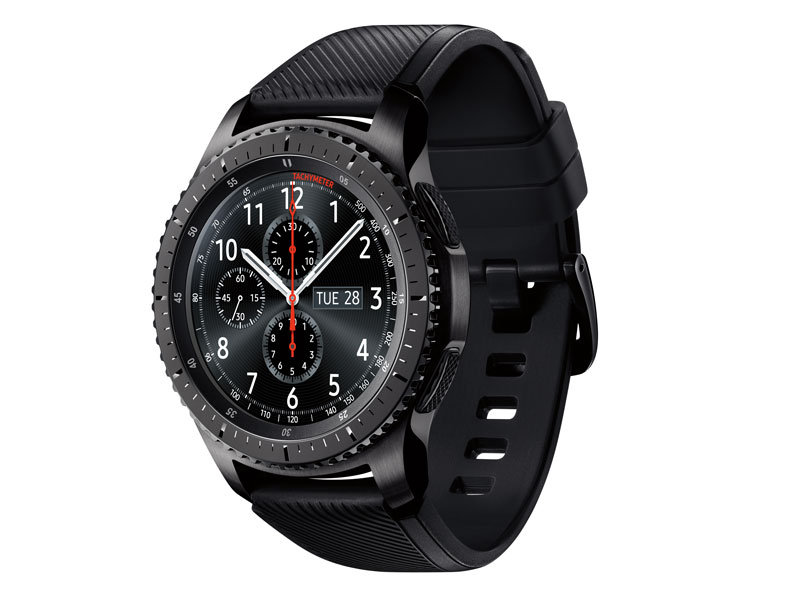
\includegraphics[width=0.5\textwidth]{samsung-gear.jpg}
	\caption{Smartwtch Samsung Gear S3 Frontier}
	\label{fig:watch}
\end{figure}

\FloatBarrier

\subsection{BITalino}

%This device was used as a mean of validating the measurements of other sensors, more specifically to provide a reference to compare with the HR estimation made by the smartwatch.

BITalino\cite{bitalinoguerreiro2013bitalino}  was used in the form of a chest band that collects various signals and sends them to the smartphone via BT. In particular it was chosen because it provides a high quality ECG signal \cite{bitalinobatista2017experimental,bitalinoguerreiro2013bitalino} that complemets the information collected by the smartwatch. BITalino was used, also, because it was a familiar tool that fitted the requirements to provide a ground truth to the other sensors used in the system. Initially the use of this device was meant to be as a validation tool and would not be used once the system was fully operational and the number of monitored patients increased. But the relevance of the information provided by the ECG signal it collected justified its presence in the context of cardiac patients monitoring.

A chest band was built in order to accommodate the sensors enumerated in \cref{table:vars} with a comfortable and practical form-factor. This was a major concern as patients comfort was very important to ensure success of the system, once it was intended to be used for long periods of time. Because of this, also battery size was an issue. Stock BITalino battery has 700mAh of capacity, but to eliminate any chance of this not being enough, a 1300mAh was used (\cref{table:battery}).

Apart from the electronic components, the chest band was built using a standard commercial chest band from Polar\textregistered  used for sports tracker devices. This was a very good base as this band had several positive aspects:

\begin{itemize}
	\item It had sown into the fabric two conductive rubber pads from which ECG could very easily be collected.
	\item Elastic and adjustable bands with easy to use locks, meaning it was very easy to put on and take off while ensuring a good fit to most patients.
\end{itemize}

To ensure protection of the electronics components, a tough fabric cover was sewn into the elastic band with holes for the on/off switch and charging port.

\begin{figure}[!h]
	\label{fig:faixa}
	\makebox[\linewidth][c]{%
		\begin{subfigure}[t]{0.5\textwidth}
			\centering
			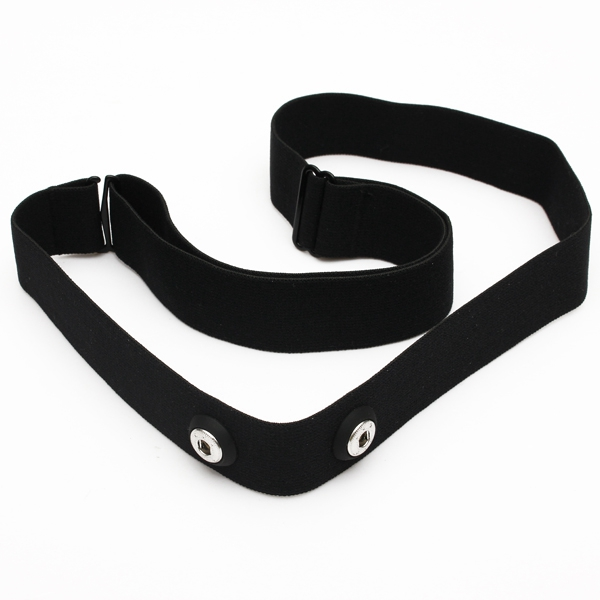
\includegraphics[width=0.8\textwidth]{faixa.jpg}
			\caption{Polar\textregistered  band that served as base for the BITalino components.}
		\end{subfigure}%
		\begin{subfigure}[t]{0.5\textwidth}
			\centering
			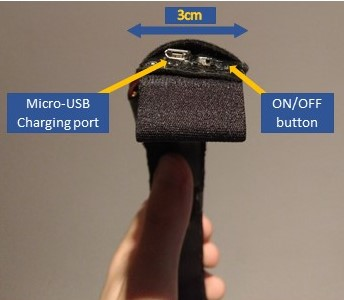
\includegraphics[width=0.8\textwidth]{faixa_botao.jpg}
			\caption{Charging port and on/off switch.}
		\end{subfigure}%
	}\\
	\caption{Chest band.}
\end{figure}

%\textcolor{red}{\Large \textbf{escala da figura esta estranha}}

\begin{figure}
	\centering
	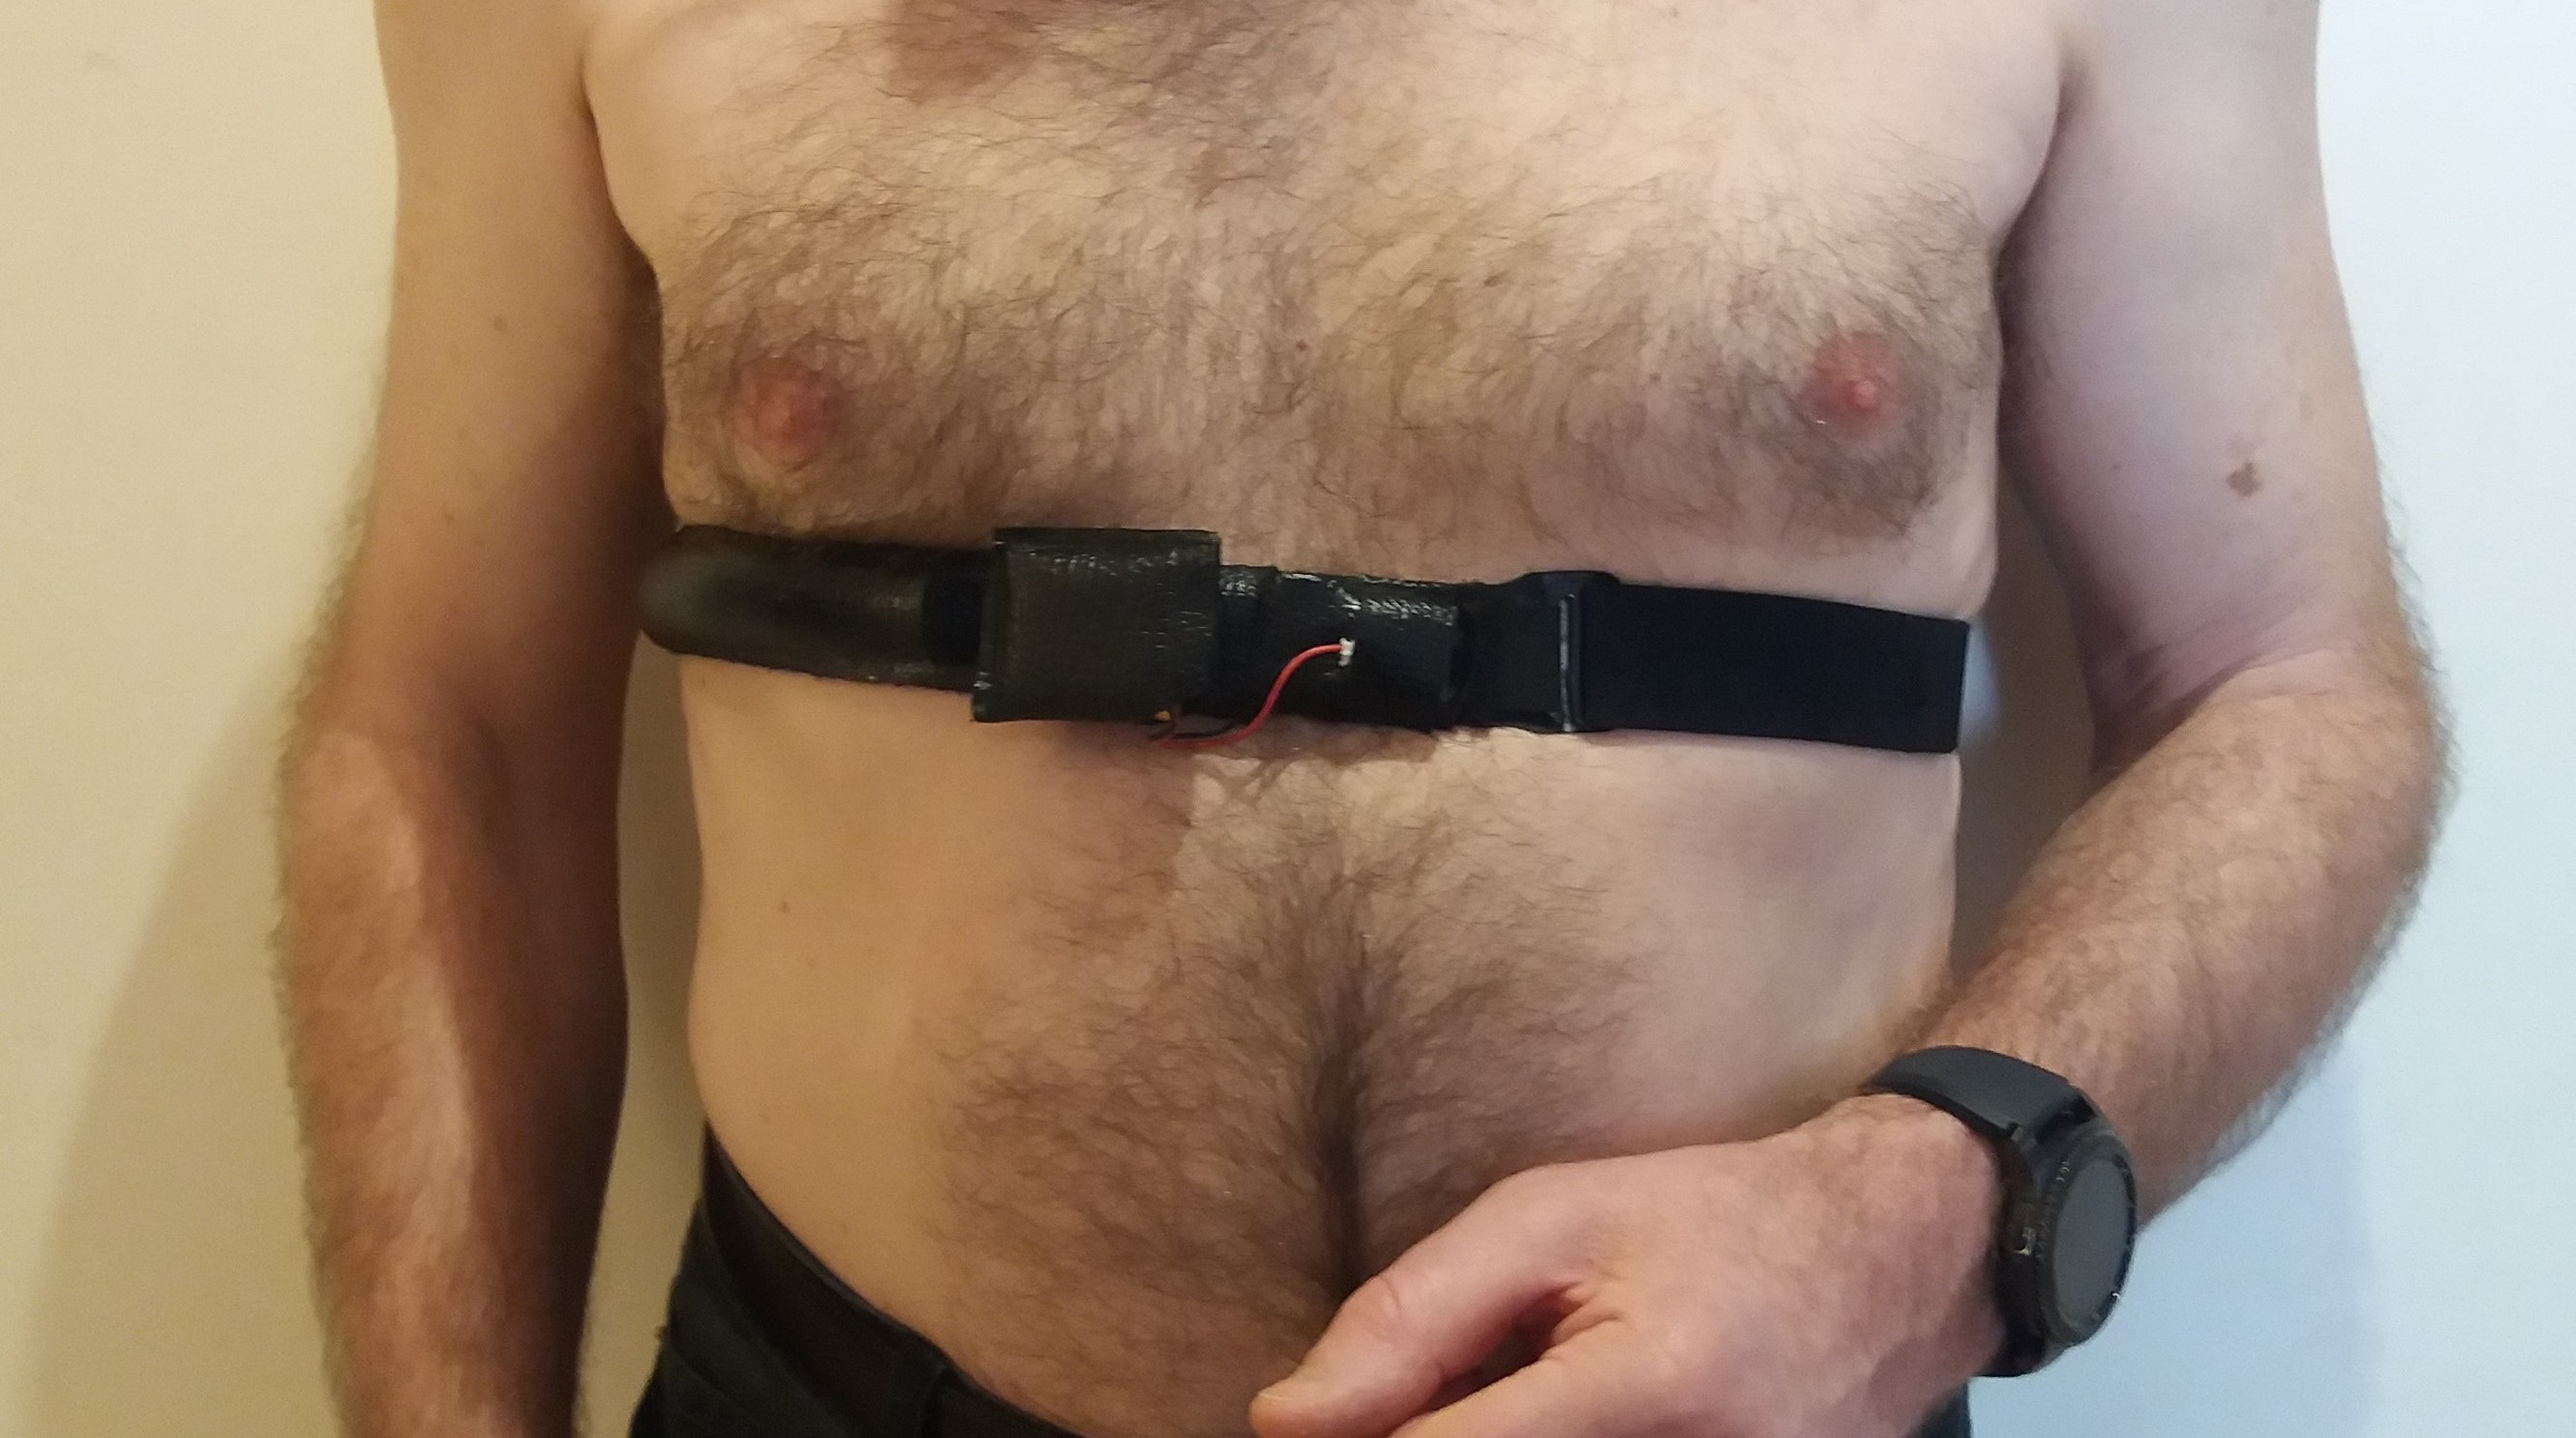
\includegraphics[width=0.6\linewidth]{setup}
	\caption{Patient wearing the selected sensors.}
	\label{fig:setup}
\end{figure}


\FloatBarrier

\section{Comfort and Usability}

As mentioned before, comfort and ease of use for patient and physician were two major concerns when designing and choosing all hardware and software features.

For the patient the importance of these aspects comes from the fact that system is meant to be used continuously for long periods of time and if the system becomes a hassle it is harder to get patient's compliance and get useful data. It was also very important that all interfaces and charging procedures were as simple as possible. This was important because great part of the patients to be monitored are elderly and in some cases even illiterate so simplicity was a major concern. For this, on screen battery information and sound notifications were utilized to notify the patient to charge the devices when needed (\cref{fig:app}).

To ensure practicality and ease of use for physicians and medical staff, requisites were to have a simple web interface (\cref{apendix:userguide}) in what concerns patient enrollment into the platform, and data visualization.

All of these aspects were assessed along the design process and were put to test in hospital context. 

During the design process students were asked to wear the system and report on aspect to be improved relating with comfort and ease of use.

As an initial hospital test, a medical team from cardiology service was given all the equipment and, using the guides provided in \cref{apendix:userguide}, fitted the system into a 72 year old male patient. Following this the patient wore the system for 24 hours and reported the experience.

From this experience the comments that emerged were mostly related with charging procedures. Web, Android and Tizen interfaces were considered very convenient and simple to use. Battery life was one of the main aspects referred as to be improved by the medical professionals. This led to the introduction of a power bank for the smartphone and a bigger battery for the chest band to ensure battery life expectations were met. Despite efforts, concerning software optimization and increased battery sizes, \cref{table:battery} still depicts slightly shorter-than-optimal battery life-times.

Another negative aspect reported was the difficulty with charging the chest band. As a safety measure, BITalino does not charge the battery while acquiring data, this was designed to guarantee isolation of the patient from the electricity mains. Although this feature creates an additional step of turning the chest band on and off when charging, the main problem reported by medical teams had to do with the toggle button. This is a very small component, as shown in \cref{fig:faixa}, which was considered difficult to use due to its size. Although it was a very valid comment, to change it, a major redesign of the chest band was required since all alternative buttons had a significantly larger size and for this reason, this aspect was left unchanged for the course of this work.

Overall the system had very positive feedback by all participants, patients and medical teams. On the medical personnel side, the system worked well as a data acquisition platform with minimum configuration required, and interfaces were considered very convenient, presenting very useful information. On the patients side there was an unexpected effect, besides considering the system comfortable to wear with minimum disturbance of their daily-life, patients reported to feel more accompanied and better taken care knowing that they are being monitored 24hr a day. This was not expected initially and may contribute to even better outcomes, as feeling more taken care of may improve patients' health status acting similarly to the placebo effect.

\begin{table}[!h]
	
	\centering
	\caption{Battery lifetime of acquisition devices}
	\label{table:battery}
	\begin{tabular}{|c|c|c|}
		\hline
		\textbf{Device}		 		&
		\textbf{Conditions}		&
		\textbf{Duration} \\ \hline
		\multirow{3}{*}{Smartphone}      &  Connected only to Smartwatch & 13h 30min  \\ \cline{2-3} 
		& Connected to BITalino and Smartwatch                                 &    11h 30min      \\ \cline{2-3} 
		& Connected to BITalino, Smartwatch and power bank                                                              &  \textbf{16h 30min}        \\ \hline
		BITalino
		& With 1300mAh battery                                                                              & 48h     \\ \hline
		Smartwatch                        & -----                                                                                             &  12h 30min        \\ \hline
	\end{tabular}
\end{table}

\section{Communications}

In order to determine if data transmission was occurring without losses nor delays, each message had a mark to allow its localization in time. For communications between the smartphone and BITalino, a sequence number is included and allows to determine if there are missing messages by checking the increment of this number. For messages between  the smartphone and Gear S3 a timestamp was sent with each message and data loses can be detected by checking the time delay between consecutive messages.

To assess the situations that led to data loss, this sequence numbers and timestamps were checked while the system was acquiring data. Distance is one of the factors that may contribute for packets being lost in transmission, although, during the normal use of the system, distances are rather short so it is not expected that this interferes with message transmission. In fact the only situation where data loss systematically occurred was when the smartphone was requesting a Bluetooth connection i.e. if the smartphone is already receiving data from device A and is trying to connect with device B, some packets coming from A are lost. Otherwise the system performed in a very robust way concerning data transmissions.

\section{Heart Rate Estimation from PPG data}

In order to evaluate the accuracy of HR estimates given by Samsung Gear S3, the later was used to record HR in different situations with several subjects with and without cardiac pathologies. Simultaneously a BITalino  \cite{bitalinoguerreiro2013bitalino} and a medical-grade certified device were used to determine the HR from ECG data and provide a ground truth reference for Gear's values.

\subsection{Methodology}

\subsubsection{Experimental Protocol}
\label{chapter:experiments}

To validate heart rate values calculated by Gear S3 three experiments were conducted:
\begin{itemize}
	\item E1 - Consisted on acquiring data for short periods of time with subjects performing a specific activity:
	\begin{itemize}
		\item Resting state, moving as least as possible (2min)
		\item Walking at a regular pace (5min)
		\item One subject was asked to pedal on a  stationary bike  at moderate pace (5min)
		\item One subject was asked to run at moderate pace (2min)
	\end{itemize}
	Some of these acquisitions were repeated to verify reproducibility and infer on system robustness.
	\item E2 - On this experiment, data was recorded for periods between 1 and 2 hours while subjects performed their usual activities during their daily lifes.
	%with 3 young healthy subjects (all 23 years old)
	\item E3 - The experiment consisted on collecting data from 3 hospitalized patients with various cardiac diseases during a stress test, taking place at hospital.
	These tests consisted of patients walking on a treadmill, increasingly fast until they are not able to continue, followed by a rest period. Patients ECG and energy consumption are monitored while executing the task. The procedure was performed according to Bruce protocol \cite{bruce}.
	%with ages (47, 42,\textcolor{red}{\Large \textbf{Idades}})
\end{itemize}


\subsubsection{Test Equipment}

Multiple devices were used to evaluate subjects' HR:

\begin{itemize}
	
	\item Samsung Gear S3 Frontier - HR is calculated by the smartwatch from PPG data using manufacturer's algorithm, as detailed in \cref{chapter:hr_bvp}.
	\item A BITalino based chest band, collecting one derivation ECG at 1000Hz, with HR estimation being made according with \cref{chapter:hr_ecg}
	\item For stress tests HR information is also collected by a Mortara XScribe 3.10.10 by Mortara Instrument \cite{mortara} that collects 12 lead ECG, producing a very reliable HR estimate as it is a certified medical device.	
	
\end{itemize}

\subsubsection{Accuracy Measurement}

The accuracy of the HR values produced by the smartwatch, and also  the ones estimated from the ECG signal, was summarized as statistics of the absolute error (AE) e.g. mean absolute error (MAE) as defined in \cref{eq:mae}.

\begin{equation}
AE_i = \left|{HR}_i^{true} - {HR}_i^{est}\right|
\label{eq:ae}
\end{equation}

\begin{equation}
MAE = \frac{1}{N}\sum_{i=0}^{N}\left|{HR}_i^{true} - {HR}_i^{est}\right|
\label{eq:mae}
\end{equation}

\begin{conditions}
	N     & nr. of HR values estimated for a subject \\
	{HR}_i^{true} 	& Ground-truth value of HR for ith 10s signal window \\
	{HR}_i^{est}    & Estimated value of HR for ith 10s signal window \\   
\end{conditions}

This measurement was chosen as it provides an easy and fast interpreting quantity to be known and used by physicians when analyzing patient data. Furthermore, unlike usual metrics like percent error, absolute error is completely independent from HR range which is a desirable feature as, ideally, the precision should be high for all HR ranges, and there is no reason for errors at higher HR values being less important.

\FloatBarrier
\subsection{Experimental Setup and Results}

Data was collected from two separate groups performing different activities. Stress tests were undertaken by 3 patients with various cardiac conditions and ages 42, 47 and 50 years old. The other experiments enumerated in \cref{chapter:experiments} were performed by 3 healthy volunteers all 23 year olds. In following figures and tables Si denotes subject i and Tj denotes jth trial.

After data collection from subjects, the first observation of the PPG signal revealed the vast influence of motion artifacts (MA). This is depicted in \cref{figure:raw}. When the subject is completely immobile it is easy to find, even by inspection, a correlation between ECG and PPG signal peaks (\cref{figure:raw_repouso}) corresponding to systolic peaks. The same is not true when the subject is moving, as signal corruption greatly affects PPG signal and correlation is no longer obvious and maybe not present at all (\cref{figure:raw_movimento}).


\begin{figure}[!h]
	\centering
	%	\makebox[\linewidth][c]{%
	\begin{subfigure}{0.5\textwidth}
		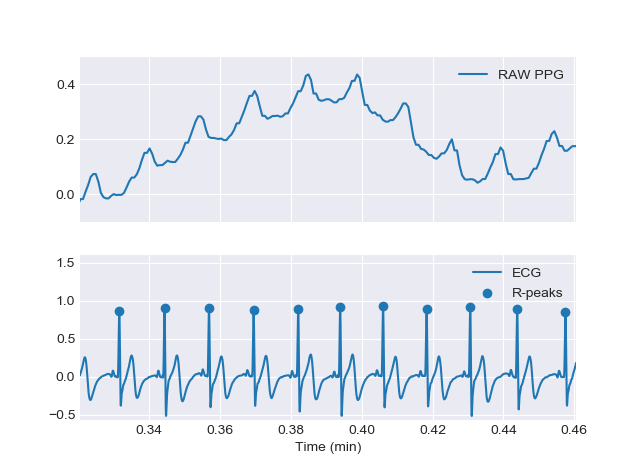
\includegraphics[width=\textwidth]{raw_repouso1.png}
		\caption{Raw signal while completely immobile. HR calculated from PPG (first curve): 75bpm; HR calculated from ECG (second curve): 79bpm.}
		\label{figure:raw_repouso}
	\end{subfigure}
	\begin{subfigure}{0.5\textwidth}
		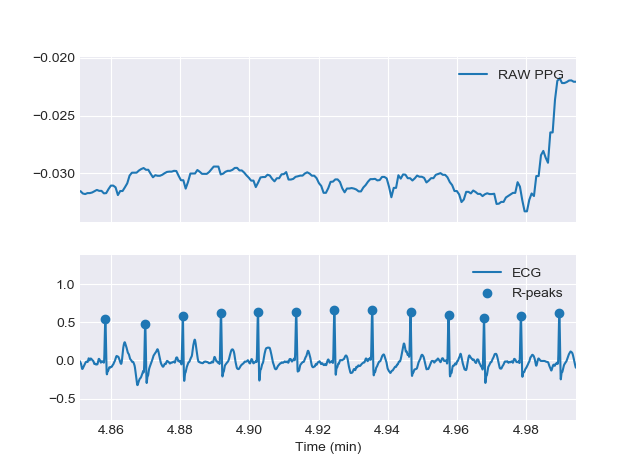
\includegraphics[width=\textwidth]{raw_movimento1.png}
		\caption{Raw signal while walking. HR calculated from PPG (first curve): 52bpm; HR calculated from ECG (second curve): 81bpm}
		\label{figure:raw_movimento}
	\end{subfigure}
	%	}\\
	\caption{Segments of raw signal captured by the sensors in different conditions with the synchronous identified R-peaks.}
	\label{figure:raw}
\end{figure}

Observing \cref{figure:hr_}, it is visible that Gear S3 is not capable of keeping up with fast variations in HR and \cref{figure:hr_hosp} clearly illustrates the difficulty in determining HR accurately during movement, with a very large estimation error being present, until subject enters the resting phase of the stress test.

%\begin{figure}[!h]
%	\centering
%%	\makebox[\linewidth][c]{%
%		\begin{subfigure}{0.45\textwidth}
%			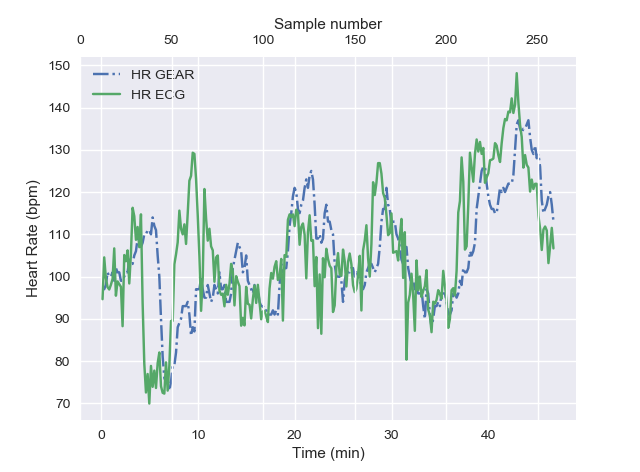
\includegraphics[width=\textwidth]{HR.png}
%			\caption{Heart Rate of subject during daily life activities.}
%			\label{figure:hr_}
%		\end{subfigure}
%		\begin{subfigure}{0.45\textwidth}
%			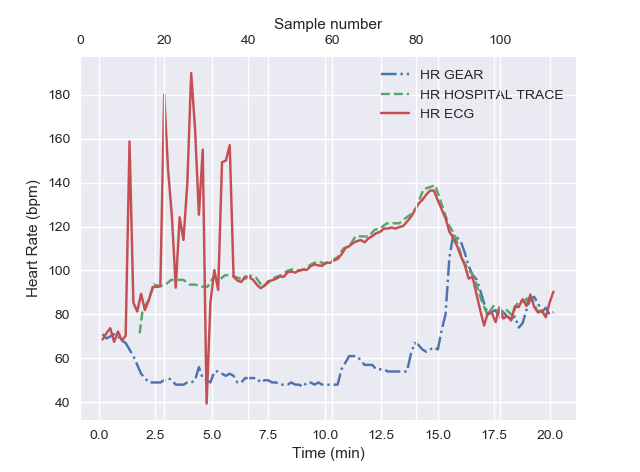
\includegraphics[width=\textwidth]{HR_hospital.png}
%			\caption{Heart Rate of subject during stress test.}
%			\label{figure:hr_hosp}
%		\end{subfigure}
%%	}\\
%	\caption{Example of HR curves obtained from  the various systems over two experiments, E1 (a) and E3 (b)}
%	\label{figure:hr}
%\end{figure}

%From the several algorithms used to process PPG data in an attempt to improve HR accuracy, none of them proved to behave better than the manufacturer's algorithm. This indicates a tailor made algorithm for this sensor in particular that is not easily replicated, even using very recently proposed state-of-the-art algorithms, as well as established methods. Having this into account, only Samsung's algorithm estimations will be considered henceforth.

%\FloatBarrier
\subsubsection{Short Acquisitions (E1)}


\begin{figure}[!h]
	\centering
	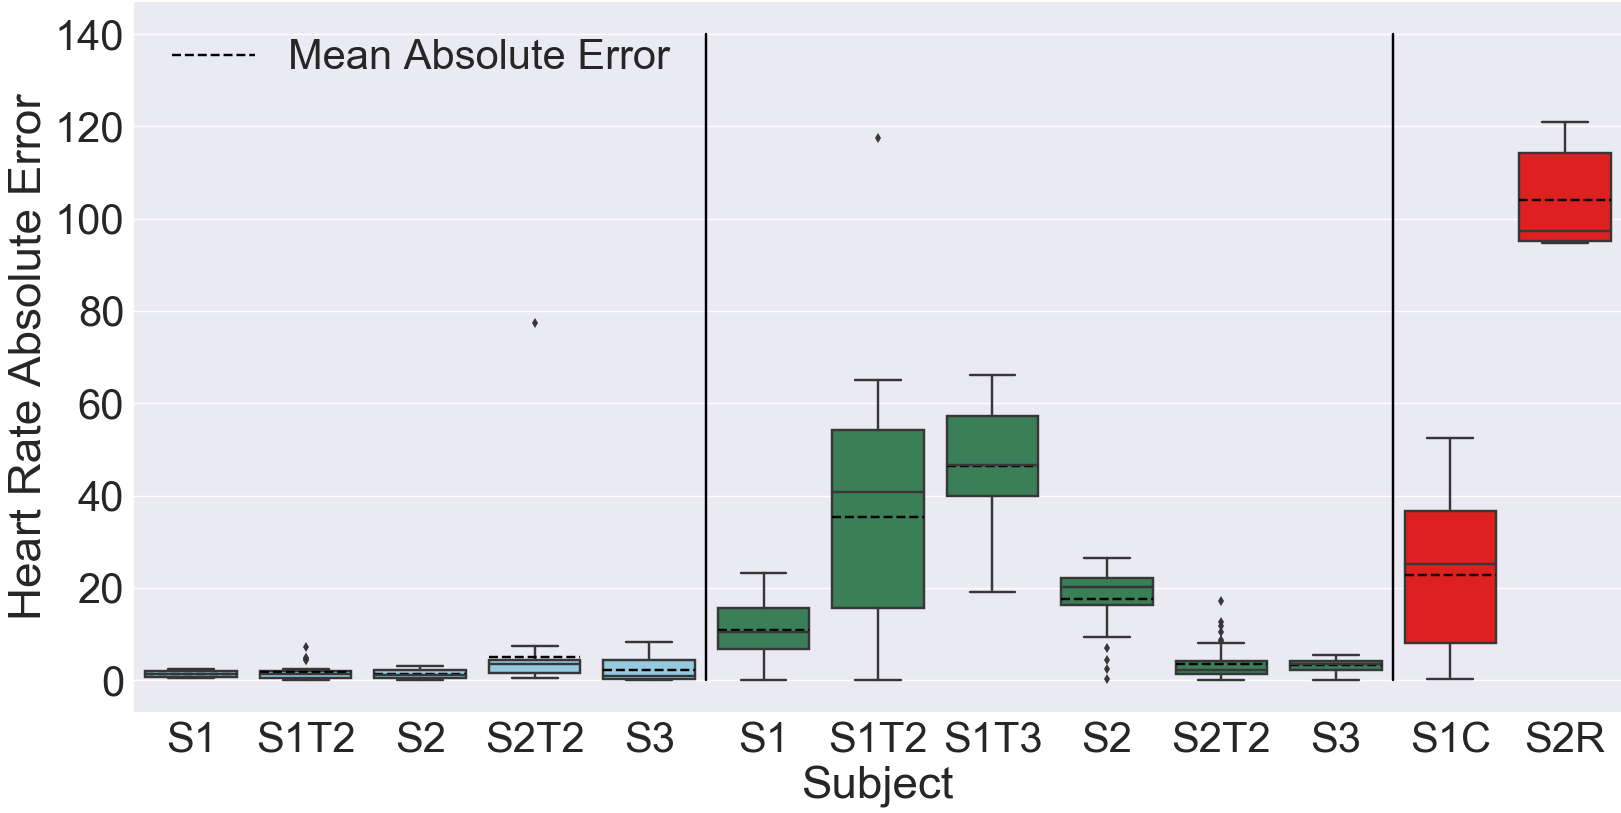
\includegraphics[width=0.85\textwidth]{box.png}
	\caption{Absolute Error of HR while performing different activities: (left) resting; (middle) walking; right cycling and running.}
	\label{figure:box}
\end{figure}

%This experiment's main activity was to determine the accuracy of the HR estimate made by the smartwatch based on the PPG data it collects, using ECG signal to provide a ground-truth.

When analyzing the absolute error of HR determined from the smartwatch's PPG data collected while subjects were performing specific activities, it is very obvious that motion highly corrupts sensor data and thus, greatly damages accuracy. In \cref{figure:box} is very clear a tendency to error increase as subjects go from resting to walking, cycling or running.
Another thing that can be noted in \cref{figure:box} and \cref{table:MAE} is the relatively large difference in the error values between subjects and trials. This may indicate low robustness of the device's measurements, as they are affected by sensor positioning, tightness and also by how the subjects move, as some individuals present accentuated arm movement which can further disrupt accuracy.

\begin{table}[!h]
	\centering
	\caption{Mean Absolute Error (MAE) of each experiment and activity averages.}
	\label{table:MAE}
	\begin{tabular}{|c|c|c|c|}
		\hline
		\textbf{Activity}                 & \textbf{Subject} & \textbf{MAE} & \textbf{Average}      \\ \hline
		\multirow{5}{*}{\textbf{Resting}} & S1               & 1.4          & \multirow{5}{*}{2.4}  \\ \cline{2-3}
		& S1T2             & 1.8          &                       \\ \cline{2-3}
		& S2               & 1.3          &                       \\ \cline{2-3}
		& S2T2             & 5.1          &                       \\ \cline{2-3}
		& S3               & 2.2          &                       \\ \hline
		\multirow{6}{*}{\textbf{Walking}} & S1               & 10.8         & \multirow{6}{*}{21.2} \\ \cline{2-3}
		& S1T2             & 35.3         &                       \\ \cline{2-3}
		& S1T3             & 46.4         &                       \\ \cline{2-3}
		& S2               & 17.7         &                       \\ \cline{2-3}
		& S2T2             & 3.4          &                       \\ \cline{2-3}
		& S3               & 3.3          &                       \\ \hline
		\textbf{Cycling}                  & S1               & 22.8         & \multirow{2}{*}{63.4} \\ \cline{1-3}
		\textbf{Running}                  & S2               & 104.1        &                       \\ \hline
	\end{tabular}
\end{table}

\FloatBarrier
\subsubsection{Daily life (E2)}
\FloatBarrier

\Cref{table:MAE_daily} and \cref{figure:box_daily} demonstrate clearly that during daily-life activities like walking or any activity that implies arm movement, Gear S3 has a poor performance as a sensor platform and, in certain occasions, it is not even possible to detect any type of signal trends. In a medical context, this could lead to gross errors when trying to diagnose or follow a patient, or it would require further tests which renders the pervasive monitoring less efficient or even counterproductive.

\begin{figure}[!h]
	\centering
	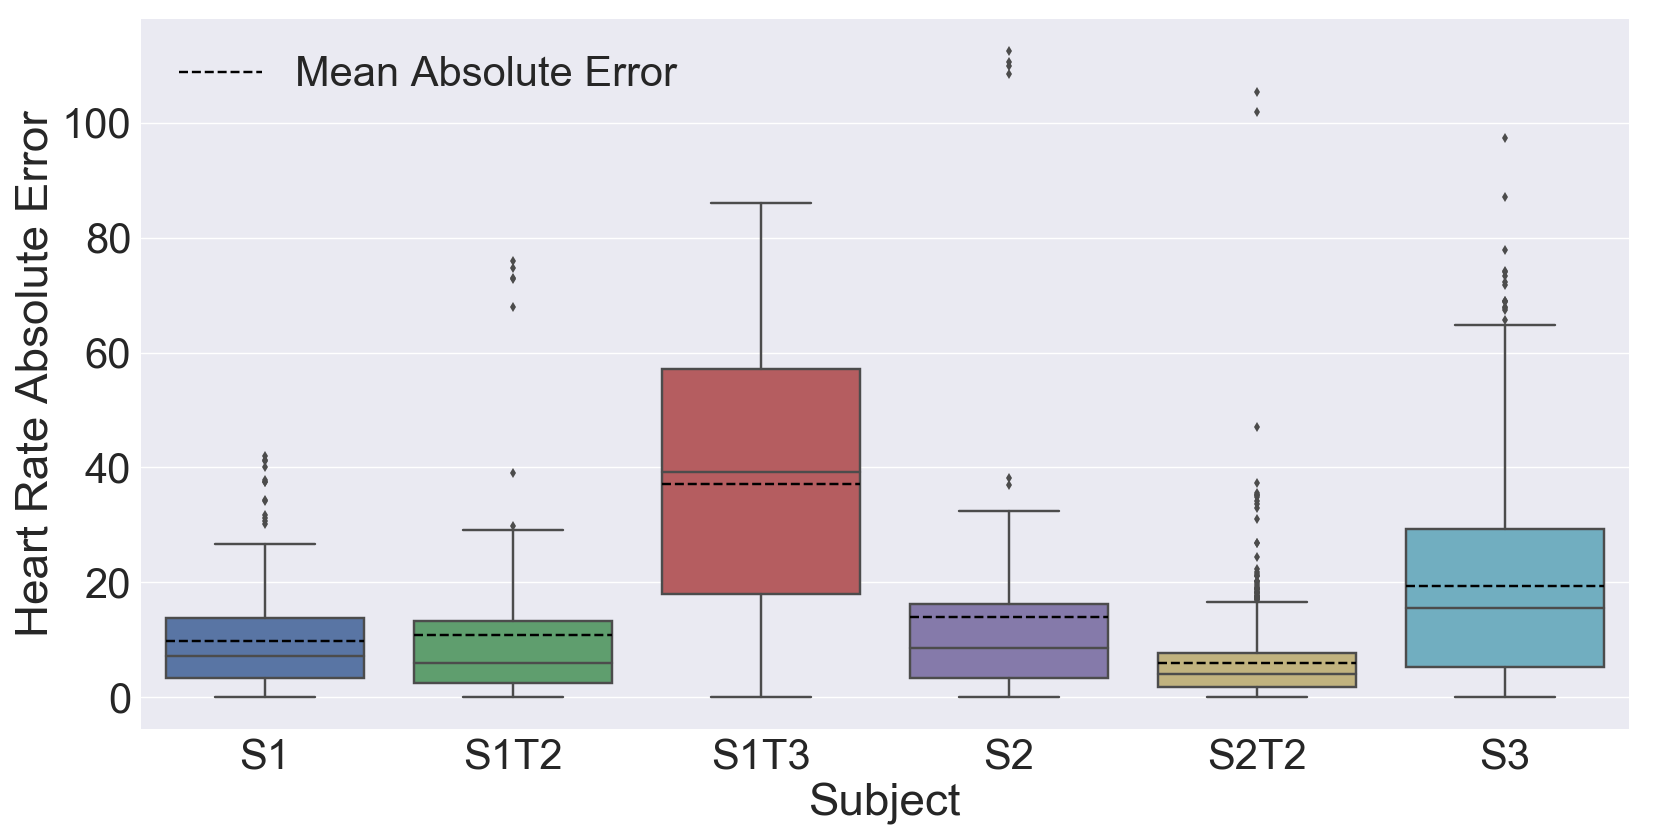
\includegraphics[width=0.85\textwidth]{box_daily.png}
	\caption{Absolute Error of HR while subjects perform their usual life activities (office working, walking, eating, etc...).}
	\label{figure:box_daily}
\end{figure}

\begin{table}[!h]
	\centering
	\caption{Mean Absolute Error (MAE) of each subject during daily life activities.}
	\label{table:MAE_daily}
	\begin{tabular}{|c|c|c|c|}
		\hline
		\textbf{Activity}                                                                         & \textbf{Subject} & \textbf{MAE} & \textbf{Average}      \\ \hline
		\multirow{6}{*}{\textbf{\begin{tabular}[c]{@{}c@{}}Daily-life\\ activities\end{tabular}}} 
		& S1               & 9.7          &\multirow{6}{*}{16.2} \\ \cline{2-3}
		& S1T2             & 10.8         &                       \\ \cline{2-3}
		& S1T3             & 37.1         &                       \\ \cline{2-3}
		& S2               & 13.9         &                       \\ \cline{2-3}
		& S2T2             & 6            &                       \\ \cline{2-3}
		& S3               & 19.3         &                       \\ \hline
	\end{tabular}
\end{table}

\begin{figure}[!h]
	\centering
	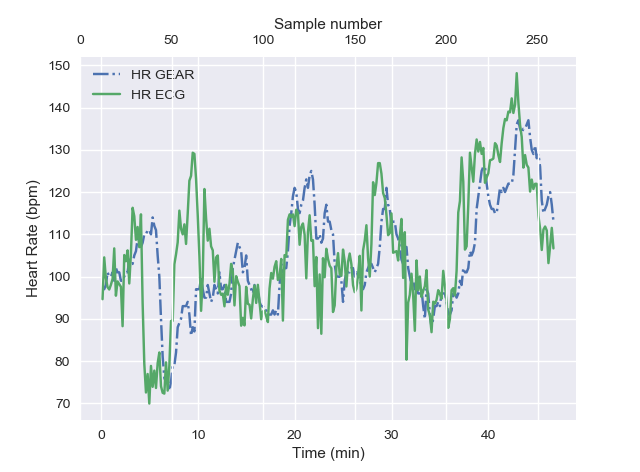
\includegraphics[width=0.85\textwidth]{HR.png}
	\caption{Example of HR curves obtained during daily life activities.}
	\label{figure:hr_}
\end{figure}


\subsubsection{Stress Test (E3)}

As expected, during a stress test, where the subject is moving with some intensity, HR determination error is very large and as can be seen in \cref{figure:hr_hosp}, error is specially large during the exercise phase of the stress test, supporting hypothesis of motion artifacts corrupting the signal.
Error during these tests reached \textgreater100bpm wich renders this sensor platform completely unfit for this kind of contextwhere precision is of utmost importance to avoid wrong diagnostics and treatments.

\begin{figure}[!h]
	\centering
	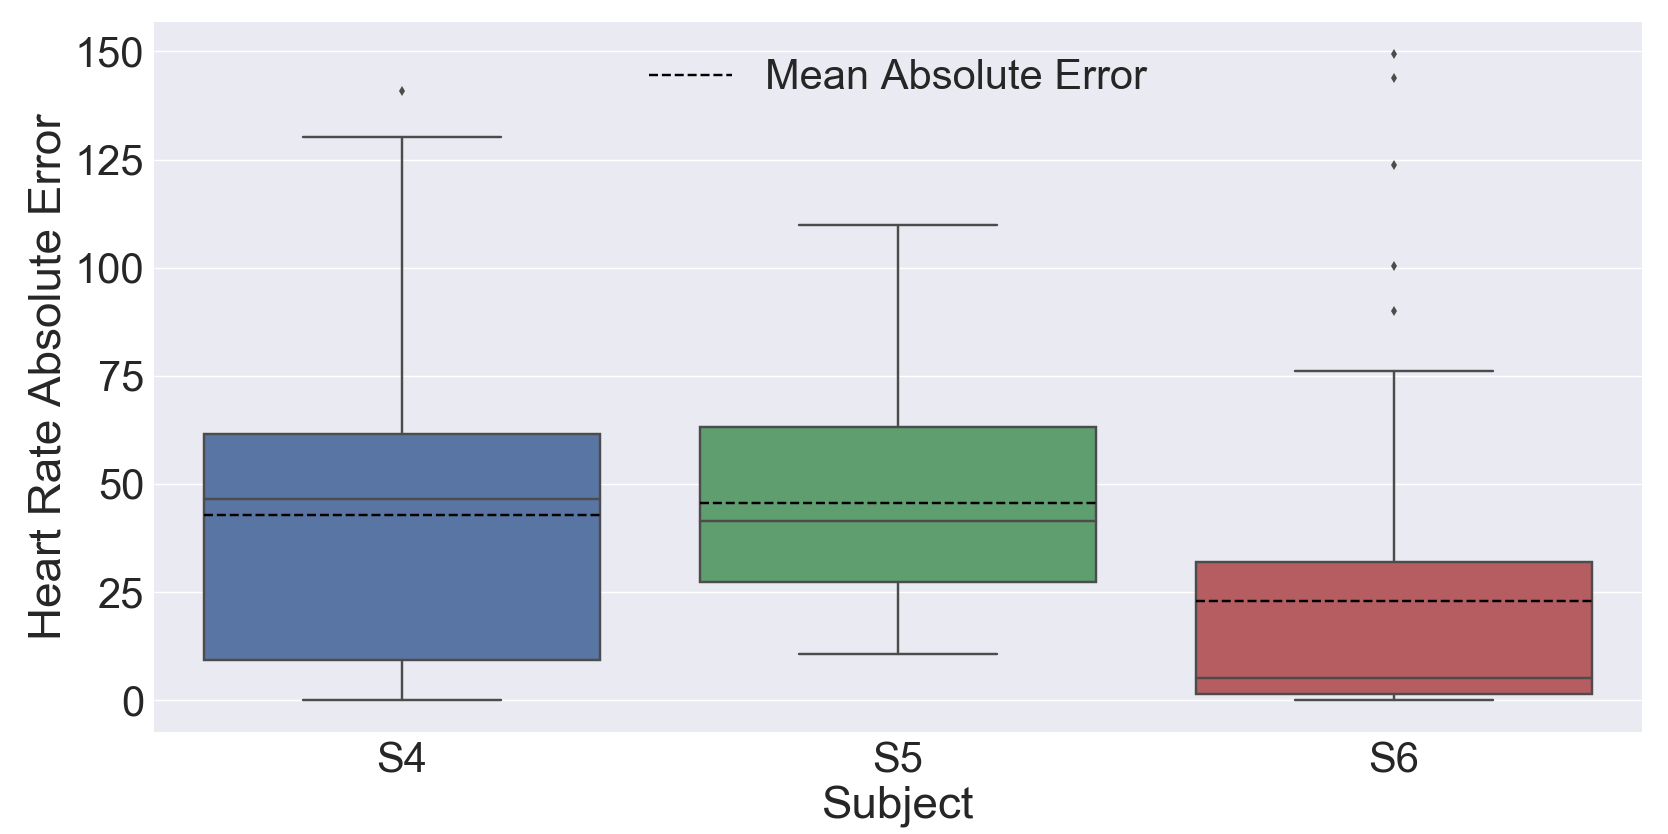
\includegraphics[width=0.85\textwidth]{box_h.png}
	\caption{Absolute Error of HR during stress test.}
	\label{figure:box_h}
\end{figure}

\begin{figure}[!h]
	\centering
	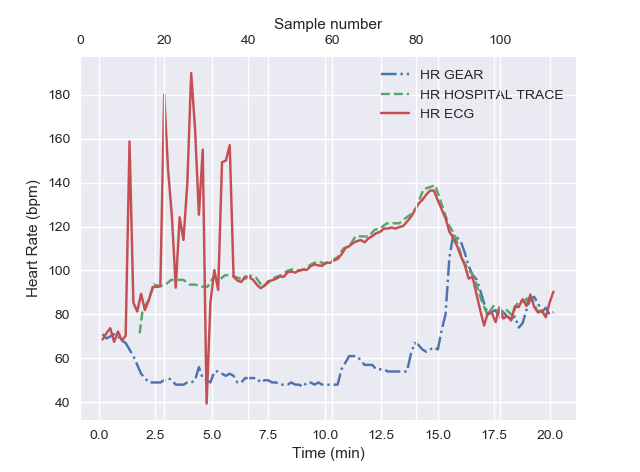
\includegraphics[width=0.85\textwidth]{HR_hospital.png}
	\caption{Example of HR curve obtained during stress test.}
	\label{figure:hr_hosp}
\end{figure}

\subsection{Discussion}

When observing the results obtained, the first conclusion that can be made is that the PPG signal collected with Samsung Gear S3 is very easily corrupted by motion artifacts. This corruption is present either during exercise or daily-life activities and even with very light movements, some corruption can be noticed. This means that very easily, the identification of systolic peaks in the signal cannot be made reliably, having a negative impact in the HR determination accuracy thus rendering this device unfit for pervasive monitoring in a medical context.

The main reasons for this low accuracy can be related with the sensor itself and also with the device as a whole. The sensor has only one green LED and one photodiode, while other sensors have two of each, with LEDs of different wavelengths. This apparent redundancy has a great impact as it allows for a different signal processing approach that can greatly improve the performance, while having only one wavelength means less information being collected, reducing the signal processing options. 

Concerning the weight, it must be taken into account that this is a very complex device that can perform endless tasks with native support for 3rd party apps. All these functionalities and capabilities make the device heavier and lager, thus, making it harder to keep comfortably and tightly secure to the wrist without it having its own dynamics. This is a problem as the relative movement between the sensor and the subject is the sole cause for movement artifacts in the signal. In addition the positioning of the sensor in an area with a relatively low SNR greatly increases the impact of motion artifacts. Also this device has the sensor at the same level of the watch back plate, whereas other devices place the sensor in an elevation of the back plate, which makes the sensor to be slightly pressed against the skin increasing SNR, and thus, accuracy. 

Due to poor quality PPG signal acquired, several algorithms were used in an attempt to get better HR estimates.
Algorithms used included adaptive filtering with and without Laguerre expansion \cite{adagibbs2005active,laguerrewood2006active}, signal separation by sparse signal reconstruction \cite{zhang2015joss,zhang2015troika} and onset detection \cite{bvponsetblazek2010multi}. A total of 8 algorithms were used to process the PPG and accelerometry data coming from S3 to produce estimates of HR. However, the results obtained using all this algorithms performed equally bad, or even worse, than Gear's algorithm and, for this reason, they were not considered. This clearly indicates that elevated error in Gear's HR estimations is probably related with a low quality signal and not with a poorly performing algorithm.

\FloatBarrier

\section{Heart Rate Estimation from ECG data}
\label{chapter:android_ecg_testing}

As a way of validating the algorithm described in \cref{chapter:android_ecg} running on the smartphone, that is being used to determine the HR from the ECG signal, a comparative analysis was made between the HR estimates based on the proposed algorithm and a standard one described in \cref{chapter:hr_ecg}.

The main difference between algorithms is that one is a very simplified RP detector running in the smartphone in real-time while the other runs off-line with no complexity restrictions.

\subsection{Methodology and Experimental Setup}

During E2, described in \cref{chapter:experiments}, ECG was collected by the chest band and was used to test the algorithm proposed in \cref{chapter:android_ecg}. At the same time, the raw signal was recorded and processed off-line by the standard algorithm. This allowed to isolate signal quality from the tests, as the same signal, divided in the same 10s windows was being processed by both algorithms and HR estimates were compared.

\FloatBarrier
\subsection{Results}

In \cref{figure:hr_android} the HR curves calculated by both algorithm can be seen. The calculations, for this particular subject, present an almost zero error, as the curves appear to be overlapping for almost all samples, and with minor deviations in a few points.

Looking at \cref{figure:erro_android} it can be noticed that observations made from \cref{figure:hr_android} are in agreement with error values for most subjects.

\begin{figure}[!h]
	\centering
	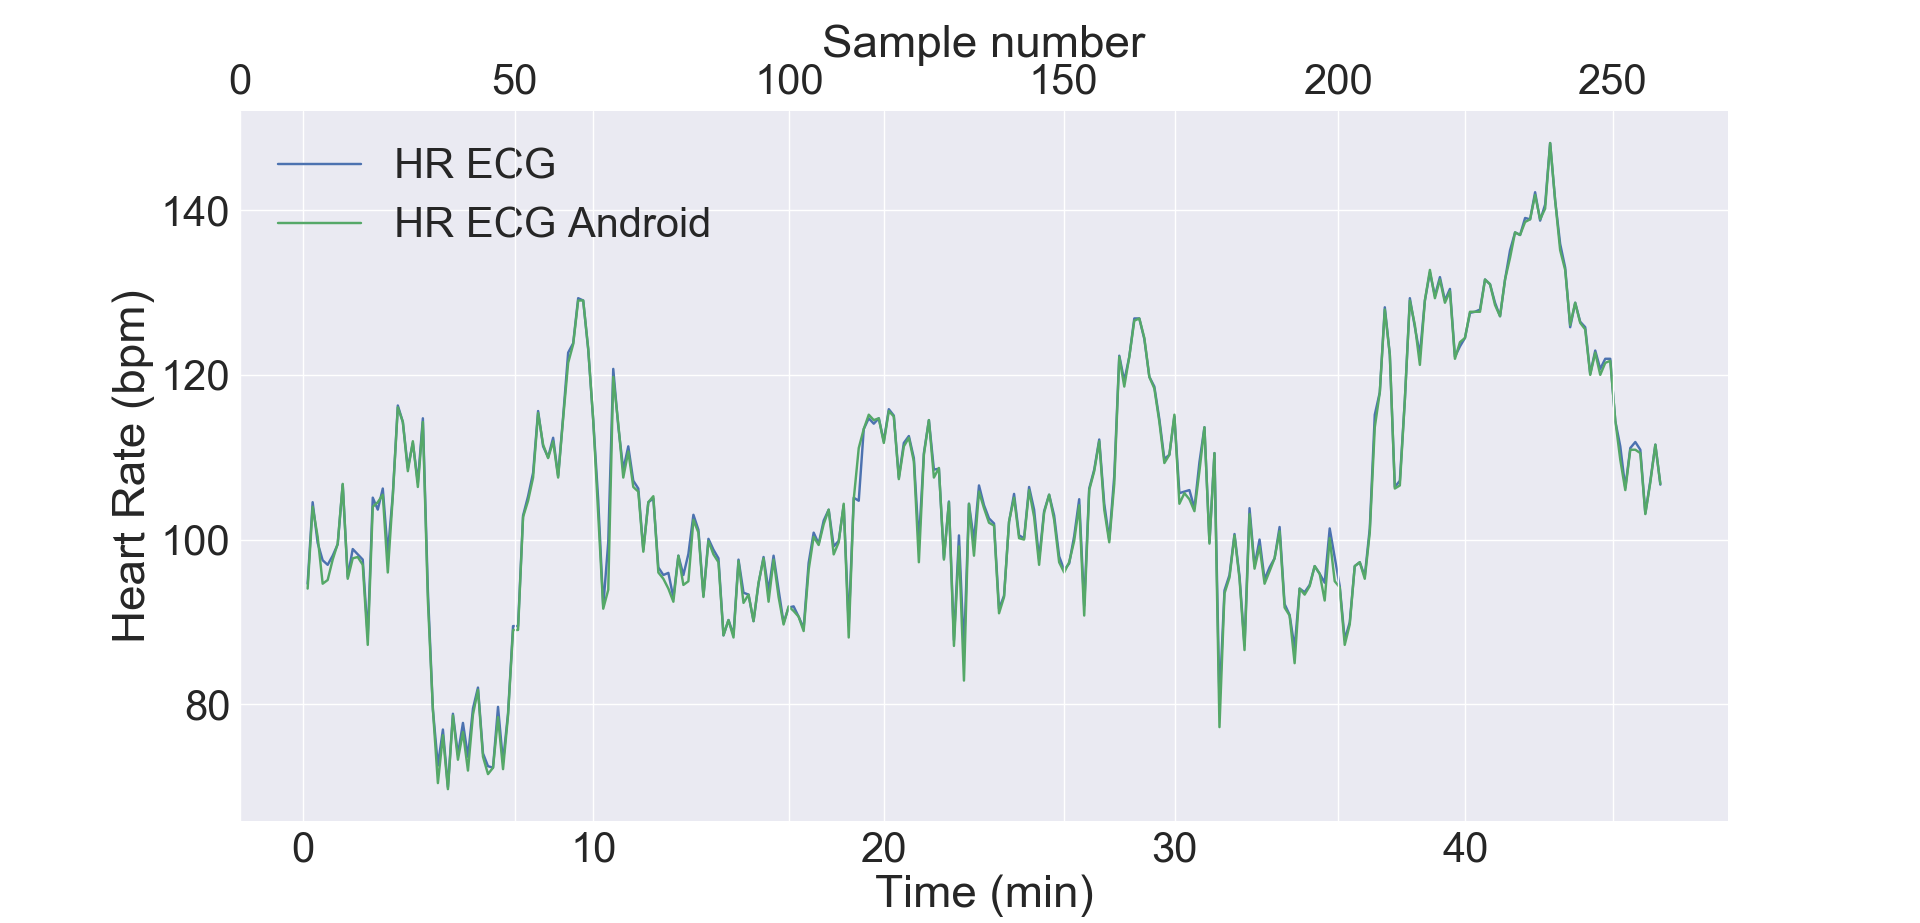
\includegraphics[width=0.85\textwidth]{hr-android-ecg.png}
	\caption{Error of android segmenter.}
	\label{figure:hr_android}
\end{figure}

\begin{figure}[!h]
	\centering
	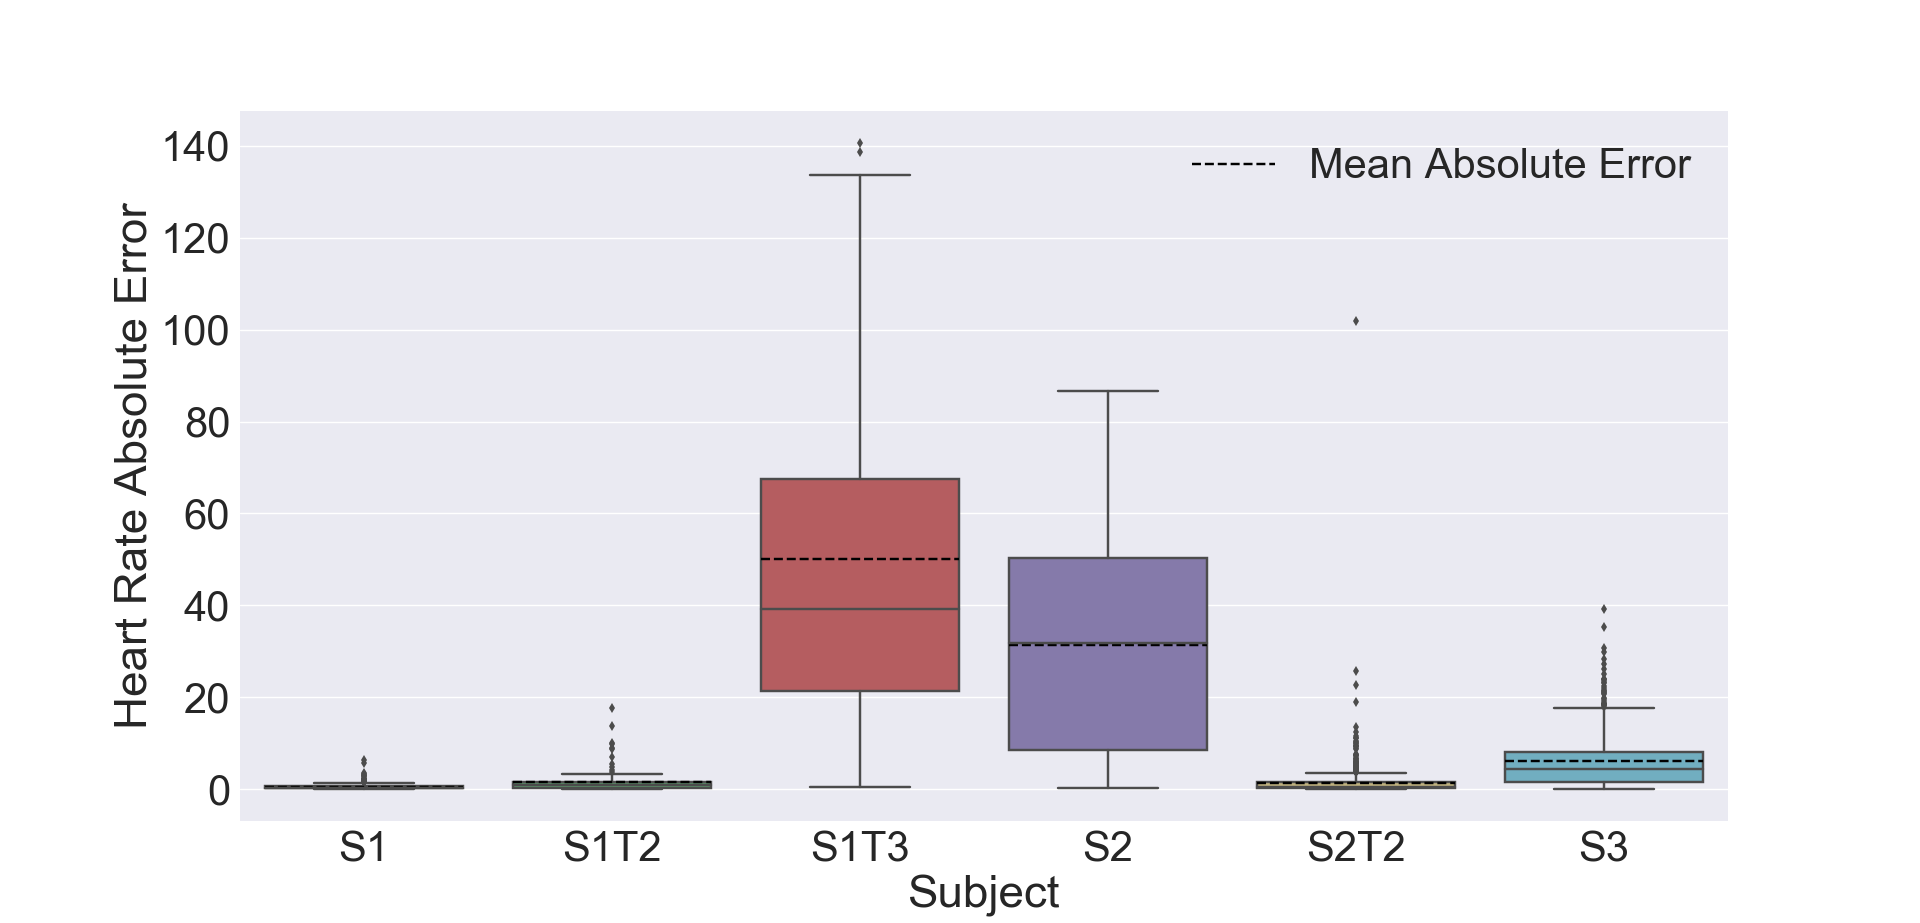
\includegraphics[width=0.85\textwidth]{erro-android-ecg.png}
	\caption{Error of android segmenter.}
	\label{figure:erro_android}
\end{figure}

\subsection{Discussion}

Analyzing \cref{figure:hr_android}, it can be noticed that HR estimation made using the proposed algorithm and the reference algoritm \cite{engzee} are rather small. This demonstrates that, even being computationally lightweight, it perform  well during daily-life tasks. Although BITalino produces a good quality ECG signal, when the wearer is moving, some artifacts are introduced, and even in this situation, HR estimates are reliable. This is confirmed by \cref{figure:erro_android}, where very small errors predominate with exception for two subjects S1T3 and S2, where Si denotes subject i and Tj denotes jth trial. In this particular pair of acquisitions, the increase of error is probably due to the introduction of motion artifacts in the ECG signal, as subjects reported to be exercising.

Besides motion artifacts, the other major weakness of this algorithm is chest band placement. This occurs due to the nature of the algorithm, as it is based in amplitude, it is expected of the R-peak to have an amplitude much larger than other signal features, which is only true for certain ECG electrodes placement. In case of a patient misplacing the chest band, it may be that signal morphology is altered leading to great errors in the HR estimation. However, with careful teaching of each patient on how to operate the system, this problem can be reduced (although not completely eliminated). To solve this problem a completely different algorithm would be needed, being, probably, much more elaborate and resource consuming.



%\begin{figure}[!h]
%	\centering
%	\makebox[\linewidth][c]{%
%		\begin{subfigure}[t]{0.55\textwidth}
%			\centering
%			\captionsetup{width=.75\linewidth}
%			\includegraphics[width=\textwidth]{hr-android-Andre.png}
%			\caption{Subject 1 HR}
%		\end{subfigure}%
%		\begin{subfigure}[t]{0.55\textwidth}
%			\centering
%			\captionsetup{width=.75\linewidth}
%			\includegraphics[width=\textwidth]{erro-android-Andre.png}
%			\caption{Subject 1 Absolute error and total accelerometry power}
%		\end{subfigure}%
%	}\\
%	\makebox[\linewidth][c]{%
%		\begin{subfigure}[t]{0.55\textwidth}
%			\centering
%			\captionsetup{width=.75\linewidth}
%			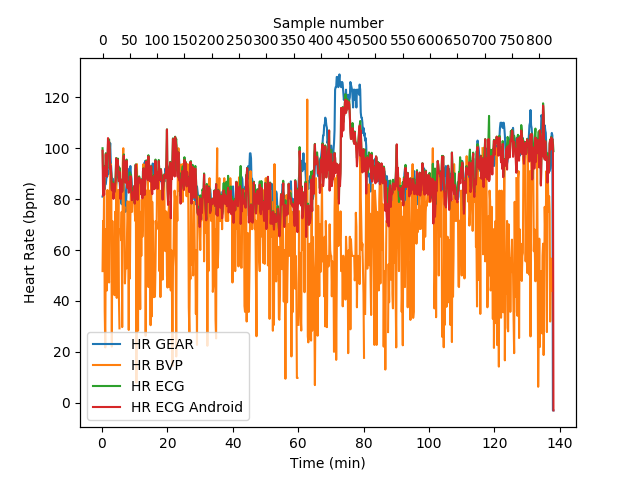
\includegraphics[width=\textwidth]{hr-android-Miguel.png}
%			\caption{Subject 2 HR}
%		\end{subfigure}%
%		\begin{subfigure}[t]{0.55\textwidth}
%			\centering
%			\captionsetup{width=.75\linewidth}
%			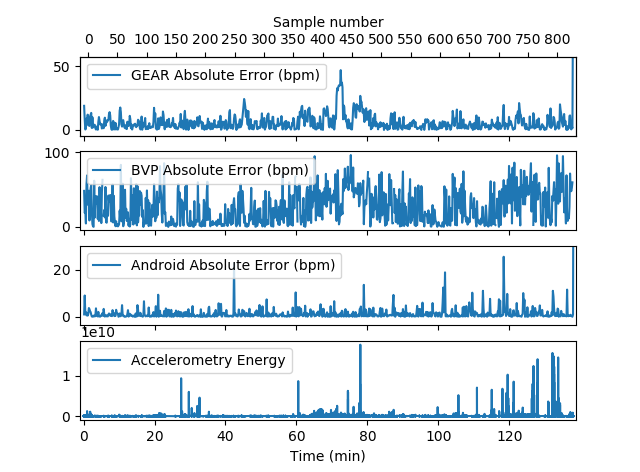
\includegraphics[width=\textwidth]{erro-android-Miguel.png}
%			\caption{Subject 2 Absolute error and total accelerometry power}
%		\end{subfigure}%
%	}\\
%	\makebox[\linewidth][c]{%
%		\begin{subfigure}[t]{0.55\textwidth}
%			\centering
%			\captionsetup{width=.75\linewidth}
%			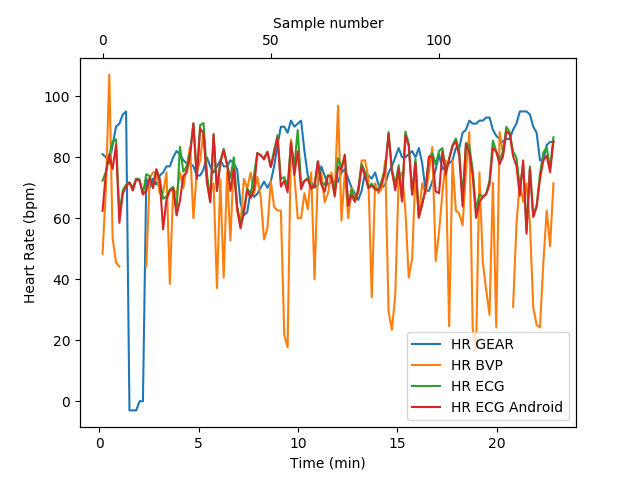
\includegraphics[width=\textwidth]{hr-android-Andre-curto.png}
%			\caption{Subject 3 HR}
%		\end{subfigure}%
%		\begin{subfigure}[t]{0.55\textwidth}
%			\centering
%			\captionsetup{width=.75\linewidth}
%			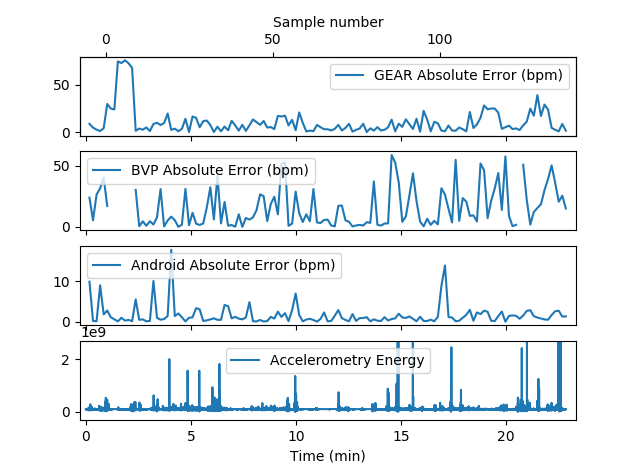
\includegraphics[width=\textwidth]{erro-android-Andre-curto.png}
%			\caption{Subject 3 Absolute error and total accelerometry power}
%		\end{subfigure}	%
%	}\\
%	\caption{\textbf{Left:} Heart Rate determined from various methods: (blue) Gear's algorithm; (orange) using BVP data and an onset detector; (red) in the computer using a state-of-the-art algorithm; (green) the proposed real-time algorithm. \textbf{Right:} Heart Rate Absolute Error from each of the methods used and Accelerometry Energy}
%	\label{fig:hr-android}
%\end{figure}
%
%\begin{table}[h]
%	\centering
%	\caption{Root Mean Squared Error \cref{eq:rmse} from each of the subjects (S1, S2, S3) and the average RMS (AV) over the three subjects, when HR is calculated either from the raw BVP signal, by the Gear or with the proposed segmenter}
%	\label{table:error-android}
%	\begin{tabular}{c|c|c|c|c|c|c|}
%		\cline{2-7}
%		& S1    & S2    & S3  & S1 (2nd)  & S3 (2nd) & \textbf{AV}    \\ \hline
%		\multicolumn{1}{|c|}{HR Android} & 0.9  & 4.4  &  3.0  &  &   & \textbf{}  \\ \hline
%		\multicolumn{1}{|c|}{HR Gear}  & 13.1 & 9.7 &  18.0 &   &   & \textbf{} \\ \hline
%		\multicolumn{1}{|c|}{HR BVP} & 56.5 & 34.5  &  21.8 &   &    & \textbf{}  \\ \hline
%	\end{tabular}
%\end{table}


Overall, the algorithm performed very well, speacially when taking its simplicity into account. Robustness may be questionable when exercising, but for daily-life activities, it is very reliable, and improving the reliability would, probably, require a great increase in the computational burden of the algorithm, harming the smartphone's battery life and the general system's usability.